% !TEX root = ../thesis.tex

\chapter{Polyhedra Analysis}
 
Polyhedra analysis is one of the main tools of static analysis. During the\\ execution of a program variables can become bounded, either by numbers or by \\other variables. Polyhedrons are one of the most expressive ways of modelling all the\\ possible values that variables can have as well as the different dependencies between them. Different alternatives exist for constraint representation instead of polyhedra, but the polyhedra domain is by far the most expressive. Unfortunately, it has worst case exponential space and time complexity meaning that using it on most real-world applications would cause it to either timeout or to run out of memory making it very impractical. Therefore, other domains have been more widely used such as octagon, zone or pentagon, but all of these are less expressive and therefore less precise by design. In the recent years several techniques have been developed that have managed to speed up polyhedra analysis without the loss of precision.

\section{Polyhedra representation}
One of these techniques involves separating the way we represent our polyhedra. Polyhedra can be represented with both their constraint representation and their generator representation. To illustrate these different illustrations I will proceed with the following example. Lets assume we have the following set of assertions:
\paragraph{Example 3.1}\mbox{}\\
\begin{center}
	$if \; x\geq0.5\wedge x\leq 1.5 \wedge y\geq 0.5 \wedge y \leq1.5: $\\
	$...\;\;\;\;\;$\\
	$end \qquad\qquad\qquad\qquad\qquad\qquad\qquad\qquad$
\end{center}

Inside of the if statement, the polyhedron would have the following shape:


\begin{center}
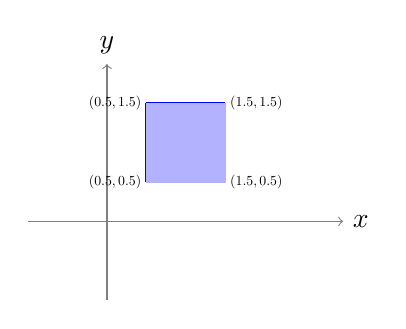
\begin{tikzpicture}
    \draw [thin, gray, ->] (0,-1) -- (0,2)      % draw y-axis line
        node [above, black] {$y$};              % add label for y-axis

    \draw [thin, gray, ->] (-1,0) -- (3,0)      % draw x-axis line
        node [right, black] {$x$};              % add label for x-axis

    \draw [draw=blue,thick] (0.5,0.5) -- (0.5,1.5)% draw the graph
   	 	node [left, black, scale =0.5] {$(0.5,1.5)$};
    \draw [draw=blue,thick] (0.5,1.5) -- (1.5,1.5)
    	node [right, black, scale =0.5] {$(1.5,1.5)$};
    \draw [draw=blue,thick] (1.5,1.5) -- (1.5,0.5)
    	node [right, black, scale =0.5] {$(1.5,0.5)$};
    \draw [draw=blue,thick] (1.5,0.5) -- (0.5,0.5)
    	node [left, black, scale =0.5] {$(0.5,0.5)$};
    	
    \draw [fill=blue!30,blue!30] (0.5,0.5) rectangle (1.5,1.5); 




\end{tikzpicture}
\end{center}
We can represent this information in two different possible ways.
\subsection{Constraint representation}
In constraint representation we model the polyhedron as the intersection of a finite number of closed half spaces and a finite number of subspace. The resulting polyhedron can be written as:

\begin{equation}
	P=\{x\in Q^n |Ax\leq b \wedge Dx=e\}
\end{equation}
where A,D are matrices and b,e are vectors of natural numbers. Therefore, the constraint representation of the above example would be:

\begin{equation}
	C = \{-x \leq -0.5,x\leq 1.5 , -y \leq -0.5 ,y\leq 1.5\}
\end{equation}

\subsection{Generator representation}
In order to encode a Polyhedron with the generator representation, we have to model it as the convex hull of three items: 

%TODO finish list with rep 
\begin{itemize}
	\item Set of vertices $V\in Q^n$.
	\item Set off rays where one end is bounded and that start from a vertex, modelling the edges of the polyhedron. 
	\item set off lines modelling the infinite edges of the polyhedron with both ends unbounded.
\end{itemize}
%TODO finish example
The result of generator representation on the previous example would have the following form: 
\begin{equation}
	G = \{ V = \{(0.5,0.5),(1.5,0.5),(1.5,1.5),(0.5,1.5)\}, R = \emptyset, Z = \emptyset \}
\end{equation}
\section{Polyhedra domain}

Now that we can represent our Polyhedra we can do some interesting calculations with them. The polyhedra abstract domain consists of the polyhedral lattice:
	$(P,\sqsubseteq,\sqcup,\sqcap,\perp,\top)$, and a set of operators that we can apply onto the different polyhedra. The different operators are the following:
	\begin{itemize}
		\item Inclusion test: $P \sqsubseteq Q$
		\item Equality test: $P=Q$
		\item Join: $P\sqcup Q$
		\item Meet: $P\sqcap Q$
		\item Widening, this operator is applied to accelerate convergence since the polyhedral lattice has infinite height:
		\begin{center}
		  \[
    C_{P\nabla Q}=\left\{
                \begin{array}{ll}
                  C_Q $ if $P=\perp ;\\
                  C'_P\bigcup C'_Q, $ otherwise$;
                \end{array}
              \right.
  	\]
		
		\end{center}

		where $C'_p=\{c\in C_P |C_Q \vdash c \}$, and\\  $C'_Q=\{c\in C_Q |\exists c' \in C_P,C_P \vdash c $ and $((C_P\c')\bigcup \{c\})\vdash c' \}$
		where $C\vdash c$, test wether c can be entailed from constraints in C
		\item Conditional: let $\otimes \in \{\leq,=\},1\leq 1\leq n,\alpha \in Q$ then $\alpha x_i \otimes \delta$ adds the constraint $(\alpha-a_i)x_i \otimes\delta - a_i x_i$ to the constraint set C
		\item Assignement: $x_i = \delta$, first adds $x_i$ to P then augments C with $x_i -\delta = 0$
		
	\end{itemize}
	 In the following table we can see the respective complexities of the different operators according to the representation
	 
\begin{center}
\begin{tabular}{||c c c c||} 
 
 \hline
 Operator & Constraint & Generator & Both \\ [0.5ex] 
 \hline
 Inclusion $(\sqsubseteq)$ & $O(mLP(m,n))$ & $O(gLP(g,n))$ & $O(ngm)$ \\ 
 \hline
 Join $(\bigsqcup)$ & $O(nm^{2^{n+1}})$ & $O(ng)$ & $O(ng)$ \\
 \hline
 Meet $(\sqcap)$ & $O(nm)$ & $O(ng^{2^{n+1}})$ & $O(nm)$\\
 \hline
 Widening $(\bigtriangledown)$ & $O(mLP(m,n))$ & $O(gLP(g,n))$ & $O(ngm)$ \\
 \hline
 Conditional & $O(n)$ & $O(ng^{2^{n+1}})$ & $O(n)$ \\ 
 \hline
 Assignment & $O(nm^2)$ & $O(ng)$ & $O(ng)$ \\ 
 
 
 \hline
\end{tabular}
\end{center}
$m=|C|,g=|G|,LP(m,n)$ is the complexity of solving a linear program with m constraints and n variables\\
As we can see no representation is faster than the other. As some operators are quicker in one but others in the other. But, as we can see in the last table, when both representations are available all operators are polynomial.\\
\paragraph{Chernikova's Algorithm} \mbox{}\\
 The first optimisation that one can do is keep both representation of the the polyhedron and for each operator picking the representation that minimises the time complexity. A conversion between the two representations is possible thanks to Chernikova's algorithm. 
 
 \section{Polyhedra Decomposition}
Another technique used increase the efficiency of polyhedra analysis, is that of online decomposition. It is based on the observation that during the execution of a program, not all it's variables are dependent on one another. Using this observation, we can separate the set of all variables into independent sets. Therefore, instead of having to represent the whole set of variables with one large polyhedron we can instead represent it with various smaller ones.\\ Let's assume we have a set of variables $\chi$ in a Polyhedron $P$. The set $\chi$ can be partitioned as $\pi_P=\{ \chi_1,\chi_2,..,\chi_r\}$, $\chi_i\subseteq\chi $. We call the partitioning of the set permissible iff $ \chi_i \cap \chi_j = \emptyset$, $ \forall i \neq j$. Once the decomposition has been done in this way, during the execution of an operator, it only has to be executed on the subset of blocks that are influenced by it. This allows for a very large performance gain. Giving us the following time complexity for the various operators.

\paragraph{Table 2} Asymptotic time complexity of Polyhedra domain operators with decomposition

\begin{center}
\begin{tabular}{||c c||} 
 
 \hline
 Operator & Decomposed  \\ [0.5ex] 
 \hline
 Inclusion $(\sqsubseteq)$ & $O(\sum_{i=1}^r n_ig_im_i)$\\ 
 \hline
 Join $(\bigsqcup)$ & $O(\sum_{i=1}^r n_i g_i m_i + n_{max} g_{max})$ \\
 \hline
 Meet $(\sqcap)$ & $O(\sum_{i=1}^r n_i m_i)$ \\
 \hline
 Widening $(\bigtriangledown)$ & $O(\sum_{i=1}^r n_i g_i m_i)$\\
 \hline
 Conditional & $O(n_{max})$ \\ 
 \hline
 Assignment & $O(n_{max}g_{max})$ \\ 
 
 
 \hline
\end{tabular}
\end{center}

 
\paragraph{Example 3.2} \mbox{}\\
Let's consider the with variables $X = \{x_1,x_2,x_3,x_4\}$ and $C = \{ x_1 + 2 \cdot x_3 \leq 10, x_2 = 1 \}$.\\
This polyhedron can be partitioned into three blocks $\pi_P = \{\{x_1,x_3\},\{x_2\},\{x_4\}\}$ and its corresponding factors are equal to:\\
$C_{P_1}\{x_1 + 2\cdot x_3 \leq 10 \} $\qquad$ C_{P_2}\{x_2 = 10 \}$
% TODO write example

\subsection{Decomposition operators}
As we change the model of our domains we must equally update the operators inside of these domains. For sake of brevity I will not go into detail about each of them, but I will only talk about the join operator as it plays an important role in the work of this paper.\\
During the join of $P$ and $Q$, most of the time their factors will not be equal$(\pi_P \neq \pi_Q)$. Therefore, we have to remake their partitions in order for their factors to be equal $\pi = \pi_P\sqcup\pi_Q$. During most joins of a normal execution this will not cause much problem, but during some cases the join can merge all blocks producing the $\top$ partition. In order to rebuild the $\top$ partition from all its blocks we use the following formula:
\begin{equation}
	P = P_1 \Join P_2 \Join ... \Join P_r = (C_{P_1} \cup C_{P_2} \cup ... \cup C_{P_1}, G_{P_1} \times G_{P_2} \times  ... \times   G_{P_r})
\end{equation}
Due to the cartesian product, building the $\top$ partition can blow up the number of generators and therefore cause online decomposition to loose its performance advantage.

\section{Reinforcement Learning for polyhedra analysis}
Both of the techniques presented in chapters 3.2 and 3.3, manage to achieve considerable performance gain without having to sacrifice any precision. Unfortunately, at some point compromises have to be made. Many different algorithms have been proposed that try their best at minimising the precision loss and maximising the resulting performance gains. \\
As explained in 3.3.1. one bad constraint can significantly decrease the performance of the whole program. The trick is being able to identify this variable at the correct time. One of the potential solutions to this problem that we shall explore in this paper is training a reinforcement learning algorithm in order to decide when to apply abstractions.

\subsection{Adapting polyhedra analysis for Reinforcement Learning}

In order to be able to apply reinforcement learning, we first have to express polyhedra analysis in terms of reinforcement learning. That is, we need an agent, a set of actions, a reward and a set of features.\\
Conceptually the problem is quite simple. We will have our agent, the static analyser, executing the analysis of a program. During analysis it will have a set of actions at its disposal. Each of these actions will have a varying performance/precision capability. The goal of the agent will be to choose the correct degree of abstraction at the correct point in time. The reward has to be some sort of compromise between the precision and the performance of the given action.

\subsection{Existing methods}
Existing methods already exploit this idea. Using techniques such as Q-learning in order to create a decision policy. Q-learning is a common linear Q-function approximation technique. However recent RL methods concentrate on the use of non-linear Q-function approximation such as neural networks. Whilst non-linear Q-function approximations have been known to be unstable or divergent in the past, development of new techniques such as experience replay has helped make them a viable tool for a series of reinforcement learning problems. In the following chapters, we shall explore the idea of using such a technique for polyhedra analysis.